\documentclass[output=paper]{langscibook}
\ChapterDOI{10.5281/zenodo.4545043}

\author{Anke Tardel\affiliation{University of Mainz} and Silvia Hansen-Schirra\affiliation{University of Mainz} and Moritz Schaeffer\affiliation{University of Mainz} and Silke Gutermuth\affiliation{University of Mainz} and Volker Denkel\affiliation{ZDF Digital} and Miriam Hagmann-Schlatterbeck\affiliation{ZDF Digital}}

\title{Attention distribution and monitoring during intralingual subtitling}  
\abstract{This paper presents results from a small pilot study carried out within the EU-funded Compass project.
With eye tracking, subtitlers' distribution of attention and monitoring during subtitling with the commercial subtitling software FAB Subtitler was investigated and analysed.
During three intralingual subtitling tasks for excerpts of German documentaries we recorded data on gaze activity of eight subtitlers.
An annotation of the created subtitles based on a comparison of the subtitles from the recording and the corrected subtitles after post-experiment proofreading allows us to link product with process data.
We found that during subtitling, attention is shifted back and forth between monitoring the content of the evolving subtitles and the timing and segmentation thereof.
Results show that subtitle reading times were longer on subtitles that were corrected during post-experiment proofreading.
In addition, we found a significant interaction with subtitle ID in that incorrect subtitles had longer reading times than correct subtitles in the beginning of the process but for subtitles created later in the session this difference was no longer significant.
This suggests that later in a subtitling session participants' monitoring capacities are impacted possibly by fatigue or cognitive overload.
In this paper, we will elaborate on the methodology and procedure and suggest interpretations and possible implications.}

\lehead{Anke Tardel et al.}
\begin{document}
\renewcommand{\lsChapterFooterSize}{\scriptsize}
\maketitle

\section{Introduction} 
Subtitling as a process, particularly intralingual subtitling for the deaf and hard of hearing (SDH), has yet to be researched more in depth with empirical methods.
In times of increasing workloads for subtitlers as well as ever-changing working environments, it becomes even more important to better understand the processes involved so we can react and adapt tools and practices accordingly.
What good is a subtitling tool if it speeds up subtitling but increases cognitive load on the subtitler and negatively influences final subtitle quality?

Established methods from translation process research such as eye tracking and keylogging seem promising to be applied to subtitling as well \citep{orrego2018using}.
These kinds of methods allow us to empirically study subtitlers' behaviour such as where they look, what and how they type, but they also help us better understand the process on a cognitive level.
Measures such as total and average fixation duration as well as fixation count are established measures to interpret cognitive load \citep{buettner2013}.
In cases where these measures can be linked to poor target text quality, e.g.
subtitles that do not comply with given standards, they inform us about failure in cognitive control mechanisms such as monitoring \citep{schaeffer-etal2019}.

In this pilot eye tracking study that was carried out within the scope of the EU-funded Compass project, we recorded subtitlers during the production of intralingual SDH for three excerpts of German documentaries to gain insights on how they interact with the subtitling software as well as implications for final subtitle quality.

\section{The intralingual subtitling process} \label{sec:tardel:2}
In subtitling for TV and film we differentiate between two main kinds of subtitling: intralingual (language of film audio matches that of the subtitles) and interlingual subtitling (film language is translated into target languages; \citealt{cintas2003audiovisual}).
What they both have in common is the translation of dialogue in audiovisual (AV) content into written content in a one- to two-line subtitle format.
Regarding the target audience, we differentiate traditional subtitles from SDH, which are typically intralingual and, in addition to the dialogue, include description of sounds and speaker identification.
Though translation studies have so far mainly focused on interlingual subtitles, due to the involved language transfer, we propose that intralingual subtitling also presents a form of translation similar to translation in easy language \citep{HansenSchirraMaass}.
In order to understand subtitling processes, it seems promising to first look into intralingual subtitling, as both intralingual and interlingual subtitling are subject to similar time-space constraints and the audiovisual content needs to be transcribed into condensed written subtitles.
To our knowledge there are no studies looking into intralingual subtitling with eye tracking.
Findings from studying intralingual subtitling and comparing them to interlingual subtitling might help in understanding how subtitling tools need to be adapted to the two forms of subtitling.

In this study, we focus on intralingual subtitling as the topic of SDH moves more and more into focus, especially after many countries across the world have passed accessibility laws (e.g.
BGG\footnote{Gesetz zur Gleichstellung von Menschen mit Behinderungen (Behindertengleichstellungsgesetz), \url{http://www.gesetze-im-internet.de/bgg/}} in Germany in 2002 or the EU Audiovisual Media Services Directive\footnote{Directive 2010/13/EU, \url{http://data.europa.eu/eli/dir/2010/13/2018-12-18}} in 2010) and regulations on the proportion of public AV content that needs to be made accessible to all target groups via subtitles, sign language or audio description.
Through the growing availability of AV content online, we see an increasing demand for subtitles. Just like the demand for translation surpasses the availability of qualified translators, this problem is no different for subtitling.
This is why the industry is constantly trying to find ways to optimise current processes by introducing assisting technology and tools with a wide range of functionalities and features.
The question is to what extent these are beneficial to the subtitling process.

Intralingual subtitling is a complex and cognitively demanding task consisting of several subprocesses; both audio and visual content need to be processed and transcribed (spoken to written language).
Similar to regular translation tasks, there is no one solution on how a translation or in this case subtitle has to look like.
Even in intralingual subtitling there are several correct subtitle renditions of the same utterance possible.
These written utterances need to follow certain standards and style guides that assure the quality and readability of subtitles for particular target groups (deaf and hard of hearing, children, language learners, etc.).
In addition, subtitles need to be synced to the timing of the audio and moving images (shot changes, banners, etc.) as closely as possible (cf. \textit{contract of illusion}, \citealt{pedersen2017far}), while at the same time bearing in mind that subtitlers are limited by the maximum reading speed of the target audience, as that often does not match the speech rate.
The reading speed controls the minimum and maximum display times of subtitles depending on the number of characters.
Especially fast-paced dialogue makes it inevitable to condense the written renditions to fit the limited one to two lines and maximum number of characters per line and subtitle.
There is usually not one correct way to subtitle: for example, whether an utterance is rendered in two separate subtitles or one two-line subtitle is up to the subtitler.

\section{Monitoring in subtitling software} 
Based on the complex nature of subtitling described in the section before, subtitling tools  feature a variety of functionalities to support the subtitler.
These functionalities range from a basic subtitle editor and video player to audio-wave display, visualisation of the ratio between number of characters and minimal reading time to error codes and subtitle overviews.
While these features are meant to assist subtitlers in their work, they also mean that subtitlers' attention needs to shift away from the audio-visual content and the subtitles themselves.
Monitoring in the subtitling task therefore goes beyond monitoring what is being typed.
In addition, subtitlers need to review the subtitles they create and monitor whether the solutions they create match the expectations, i.e. style guide.
For the purpose of this study, we adopt Kitchener's second level of cognitive processing.
While the first level refers to the cognitive tasks involved, which in the case of subtitling include, e.g., listening, watching, and reading, Kitchener's second-level concept of monitoring as a meta-cognitive activity is defined by “processes which are invoked to monitor cognitive progress” \citep[225]{kitchener1983cognition}.
This model of monitoring “account[s] for complex monitoring when individuals are faced with ill-structured problems” \citep[222]{kitchener1983cognition}.
In the case of our study, errors in subtitles, i.e. subtitles that need to be adapted to comply with a given style guide, can be regarded as such ill-structured problems triggering monitoring processes while working on them.

Innovative subtitling software attempts to assist subtitlers in solving these ill-structured problems to minimise the cognitive load, e.g., in helping the subtitler apply subtitling strategies to comply with the style guide.
Common features of these subtitling tools include a video player and subtitle editor as well as an overview of all the subtitles in a file.
Usually, in and out times as well as the sequential subtitle ID and subtitle duration are displayed on screen as well.
Many tools also visualise the audio in waveform to easily navigate in the video and support subtitle spotting, i.e. setting the in and out timestamps of subtitles synchronously to when speakers start or end their dialogue.
Commercial tools can display an additional ``time bar'' that indicates the proper subtitle display time per number of characters, and error codes are displayed on-screen when a subtitle is too long or short, etc.
The list of visual features a subtitler is faced with during the task of watching the video and reading the subtitle text as it is produced is long.
Features are used successfully and monitoring can be assumed to have worked well when the produced subtitles no longer contain style guide-related errors.
If this is not the case, the visual features are either not used properly or the distribution of attention on so many different areas leads to the result that something is overlooked, i.e. monitoring fails.
In SDH, there is a thin line between rendering and describing everything and risking to lose the target audience and censoring or patronising the target audience by condensing information or changing relevant information.
So there is always the possibility that even if the style guide is being followed, the target audience might not like it.
Identifying indicators for when monitoring in subtitling fails can help adapt subtitling tools and develop strategies.

Based on the many aspects subtitlers need to monitor during subtitling, we propose the following research questions:

\begin{description}
  \item[RQ 1.] How is attention distributed on the user interface in the subtitling tool during intralingual subtitling?
  \item[RQ 2.] How is attention distribution and monitoring of one's own subtitling related to the final subtitle quality?
\end{description}

\section{Data and method}
The study applies two methodologies, keylogging and eye tracking, but in this paper only the eye tracking and product data are analysed.
We applied these methods to the subtitling process, similar to the study done by \citet{orrego2018using}, who observed interlingual subtitling processes of students and professional subtitlers working with and without transcript.
In our study, however, we observed the intralingual subtitling process and recorded behavioural and product data with these methods.
Demographic data and information on participants' use of subtitling tools were recorded with a follow-up questionnaire.

\subsection{Participants}\label{sec:tardel:4.1}
The participants ($N=8$, all female) in this pilot study were experienced subtitlers ($\text{mean} =3.5$ years) at a German broadcasting company with German as their native language.
Four of the participants are regular employees who have been working as subtitlers at the company for an average of 5 years ($\SD=2.5$) and most of their work ($80\%$) consists of proofreading subtitle files.
The other four participants are experienced students with 2.3 years' ($\SD=1.3$) professional experience in intralingual subtitling.
All eight participants are familiar with FAB Subtitler Standard as subtitling tool and work with it on a regular basis.
Though the majority of the work is for productions of German TV broadcasters with their own set of subtitling rules, all subtitlers were somewhat familiar with the Netflix timed text style guide \citep{netflix2018timed} as many productions, especially documentaries, are subtitled for Netflix.
We chose the Netflix timed text style guide general requirements (ibid.) and the supplement for German as it is internationally used and provides a rather strict set of rules.

\subsection{Procedure} 
Participants were recorded creating German SDH for three video snippets from German documentaries using the stand-alone subtitling software FAB Subtitler (Standard Edition).
The initial aim was to observe subtitlers while using a subtitling tool they were using on a regular basis and to study the distribution of attention.
For this purpose, we divided the tool into areas of interest (AOI) that represent a specific feature or functionality in the tool.
Important AOIs include:

\begin{itemize}
\item the subtitle editor (current subtitle, CS)
\item the video player
\item audio track with subtitle in and out indicators overlaid
\item reading speed control bar, i.e.
time bar (characters/subtitle duration)
\item subtitle navigation on the right-hand side
\end{itemize}
All AOIs were labelled the same in all recordings except for the AOI of the current subtitle (e.g.
CS46) which matched the ID of the subtitle that participants currently worked on.
All numbered CS AOIs were grouped as CS in order to compare this AOI to the other AOIs in the overall process.
An overview of all AOIs is given in Figure~\ref{fig:1_AOIs}.

\begin{figure}
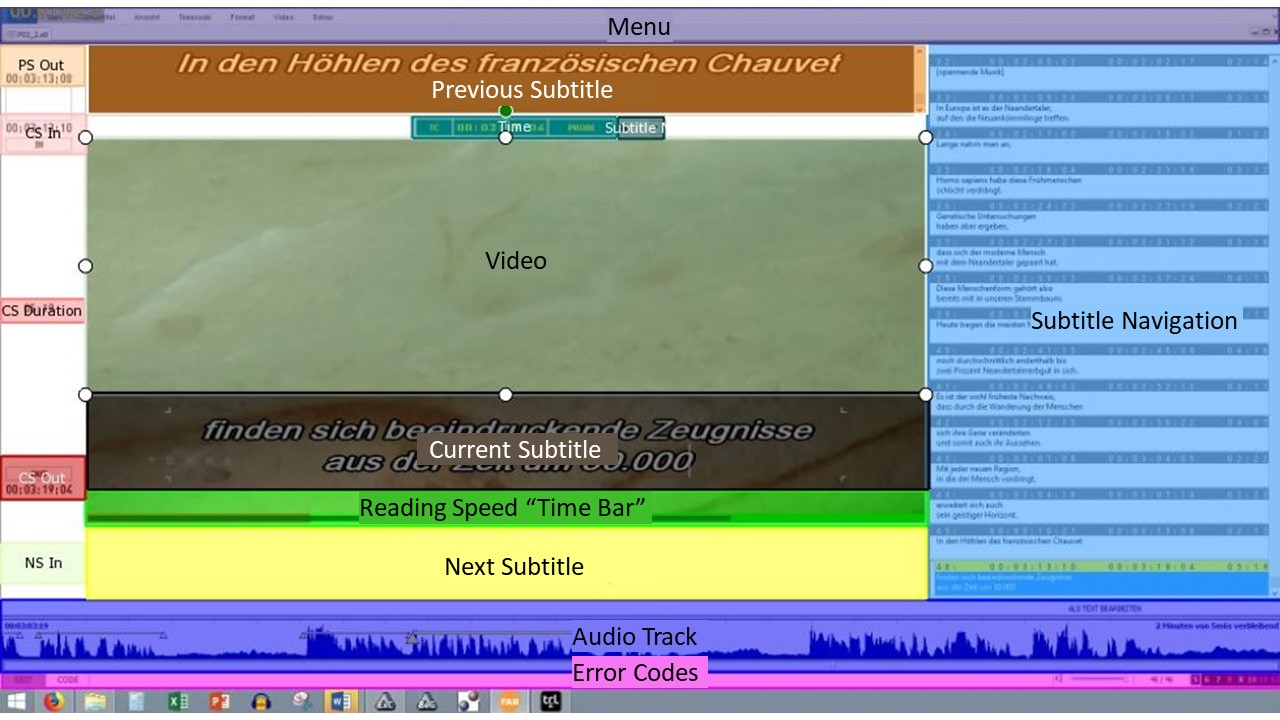
\includegraphics[width=1\textwidth]{figures/AOIs_2.jpg}
\caption{Screenshot of FAB Subtitler user interface with labelled AOIs\label{fig:1_AOIs}}
\end{figure}

The tool was configured for the Netflix timed text style guide and participants were able to use the browser for external research and checking the style guide.
The subtitling brief included the instruction to create German SDH according to the style guide.
Subtitling was done from scratch, i.e.
aside from the style guide and web browser participants had no additional reference material, no assistance via a script or automatic detection of shot changes.
All eight participants subtitled all three videos in a randomised order.
Before the first recording, subtitlers performed a copying task to record typing speeds.
Individual subtitling sessions lasted about an hour per video.
The videos were controlled for their length (five minutes) and topic.
They were taken from the German documentary series \textit{TerraX} covering topics such as anthropology, archaeology, history and architecture.

Participants performed the tasks during their regular working time in their regular work environment on a laptop equipped with an eye tracking device.
Eye movements were recorded with an SMI RED mobile eye tracker (250\,Hz) and screen recording in SMI Experiment Center.
Participants were seated at approximately 60\,cm from the eye tracking device where their eyes were calibrated (5-point calibration) before the beginning of each recording session and then every 15 minutes during the recording to avoid drift.
After the third recording, participants filled out a questionnaire to collect demographics and data on their usage of the tool.
Based on feedback from the subtitlers who participated in this study, we learned that it is common practice to distribute the subtitling work for an hour-long video or episode among three to four subtitlers, each subtitling a section of fifteen minutes.
Splitting the work between subtitlers is a practice to meet the tight deadlines as the time spent on a one-hour video can be reduced and coherence is ensured in the overall proofreading of all parts by one proofreader.
The experiment design of three five-minute video excerpts therefore seemed realistic enough.
On average, intralingual subtitling of a five-minute documentary without any further assistance by a transcript or automatic detection of shot changes takes about an hour.
This is already rather long for an eye tracking study and had to be accommodated for with repeated calibrations.

Half a year after the initial recording, the four subtitlers who usually perform the proofs were given the subtitle files for blind proofreading.
The six-month time-lag was necessary so the subtitlers would not remember having subtitled the excerpts before.
The proofread subtitle files were then compared to the subtitles created during the experiment and annotated for timing errors, linguistic errors and style-guide-related errors.
The annotation is based on what proofreaders corrected and the timing configurations regulated by the Netflix style guide.
There was no process data recorded on the proofreading and it is just one proofreading per target text, i.e. subtitled excerpt.
This adds to the ecological validity of this study as this is how quality assurance is done in the broadcasting company where we recorded the subjects.

Subtitling quality is another complex and to this point often debated concept which will not be further discussed in this paper.
We therefore only looked at the broad distinction between correct and incorrect subtitles, leaving error types and weighting of errors aside for now.
Whether a subtitle was correct or incorrect is based on the proofread versions.
No edits meant a subtitle was correct, whereas changes made to the subtitle indicated an incorrect subtitle.
There was no particular pattern regarding how errors were distributed within and across the three videos.
An overview on how errors were distributed can be found in Figure~\ref{fig:2_errors}.

\subsection{Measures}
During the subtitling task, both product and process data were recorded for all sessions, i.e. three sessions per participant.
Regarding the process data, in this analysis, we focus on the eye tracking data.
The two gaze measures of interest in this analysis are \textit{average fixation duration} on an AOI, e.g.
the current subtitle and \textit{total fixation duration} which indicates the sum of all fixation durations on an AOI.
In the case of the subtitle AOI the total fixation duration is the total reading time (TRT).
Longer average fixation duration are taken to indicate higher cognitive effort, i.e. longer processing.

For the product data, the final subtitle files were analysed and annotated with the following parameters:

\begin{description}
\item[ID:] the sequential number of a subtitle, used to align process data from the AOIs with the product data from the subtitle files. As the subtitling process is chronological, lower ID indicates the subtitle appeared earlier in the video and was therefore created early in the process (per recording).
\item[CharCount:] the number of characters in a subtitle, irrespective of the number of lines in a subtitle.
\item[CharDiff:] the difference between the maximum number of characters in a subtitle and number of characters. The maximum number of characters is determined by the Netflix style guide configuration set in FAB.
\item[Timing:] if the \textit{CharDiff} in a subtitle is negative by more than three characters, i.e. the subtitle contains more than three characters too many for the set display time of the subtitle, the subtitle was annotated with \textit{Err}, i.e. the timing is incorrect. Subtitles with an excessive display time were not penalised.
\item[Text:] subtitles were annotated with \textit{Err} whenever a subtitle was edited during post-experiment proofreading. In this variable, the type of edit was not distinguished, and unedited subtitles were annotated with \textit{Cor}.
\item[Proof:] indicates whether a subtitle is correct (\textit{Cor}) or contains an error (\textit{Err}), i.e. the subtitle contains an error either in \textit{Timing} or \textit{Text}.
\item[ErrorType:] Indicates the nature of the error in \textit{Proof}.
We differentiated between errors of \textit{Ling} (language-related, e.g.
grammar, punctuation or terminology), \textit{Style} (style guide-related, e.g.
segmentation, numbers and units, labelling) and \textit{Timing}.
\end{description}

\begin{figure}
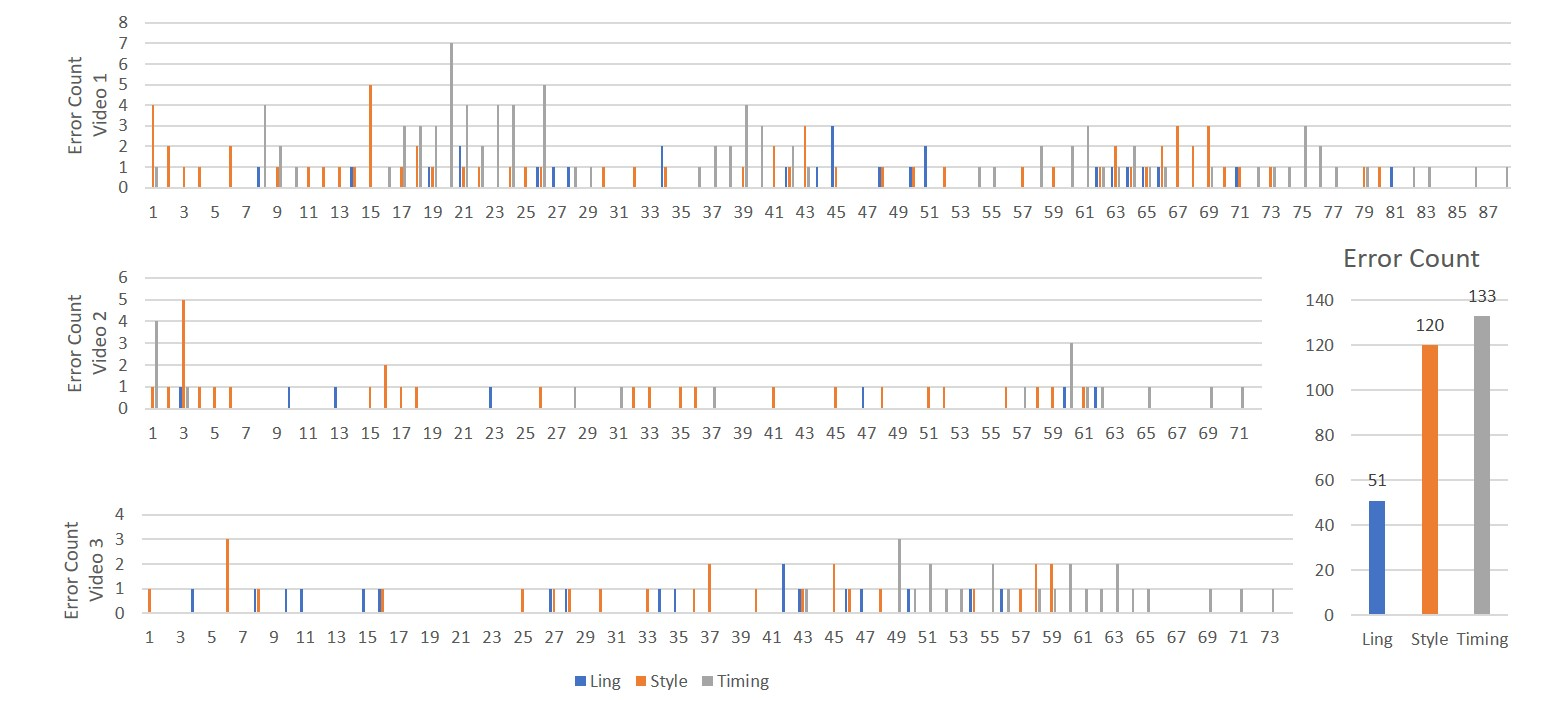
\includegraphics[width=1\textwidth]{figures/ErrorDistribution.jpg}
%\includesvg[width=1\textwidth]{figures/ErrorDistribution.svg}
\caption{Distribution of errors per subtitle ID and video across participants.
Errors are divided into the three error classifications Ling, Style and Timing.\label{fig:2_errors}}
\end{figure}

The diagram in Figure \ref{fig:2_errors} shows how errors were distributed per video and subtitle ID.
Here, we see that there was no pattern whether errors occurred early or later in a session and there was also no pattern for the different error types.
Video 1, however, seems to contain more errors in total than the other two videos.

\subsection{Data analysis}
For statistical analysis of the data we used R, version 3.6.0 \citep{R}.
Linear mixed effects models (LMEs) were fitted with the packages \texttt{languageR} \citep{baayen2019package}, \texttt{lme4} \citep{Bates2015lme4}, and \texttt{lmerTest} \citep{Kuznetova2017lmerTest} was used to calculate significance values.
To support the interpretation of the models, the effects were visualised in effects plots using the \texttt{effects} package \citep{Fox2009effects}.
Contrasts within a model were calculated with the package \texttt{emmeans} \citep{lenth_emmeans_2019}.
The LMEs were all fitted with one of the process-related measures as dependent variable and participant as random variable.
Dependent variables were not log-transformed.

\section{Results} 
\subsection{Attention distribution}
As described in \sectref{sec:tardel:2}, the task of intralingual subtitling is rather complex and involves various subprocesses, such as watching the video (images and shot\linebreak changes) while listening to and understanding the audio (dialogue and sounds) and keeping an eye on the timing as well as spatial limitations of the subtitle that is created.
Modern subtitling software contains a number of features to support subtitlers in this complex process, among them a video player, subtitle editor, audio track, etc.
For a screenshot of the user interface of FAB Subtitler refer to Figure \ref{fig:1_AOIs}.
We assume that, during the subtitling, the subtitlers' attention is divided between the various windows and functions onscreen but also the audio.
Thus, our first research question was: how is attention distributed on the subtitling tool during intralingual subtitling?

\begin{figure}
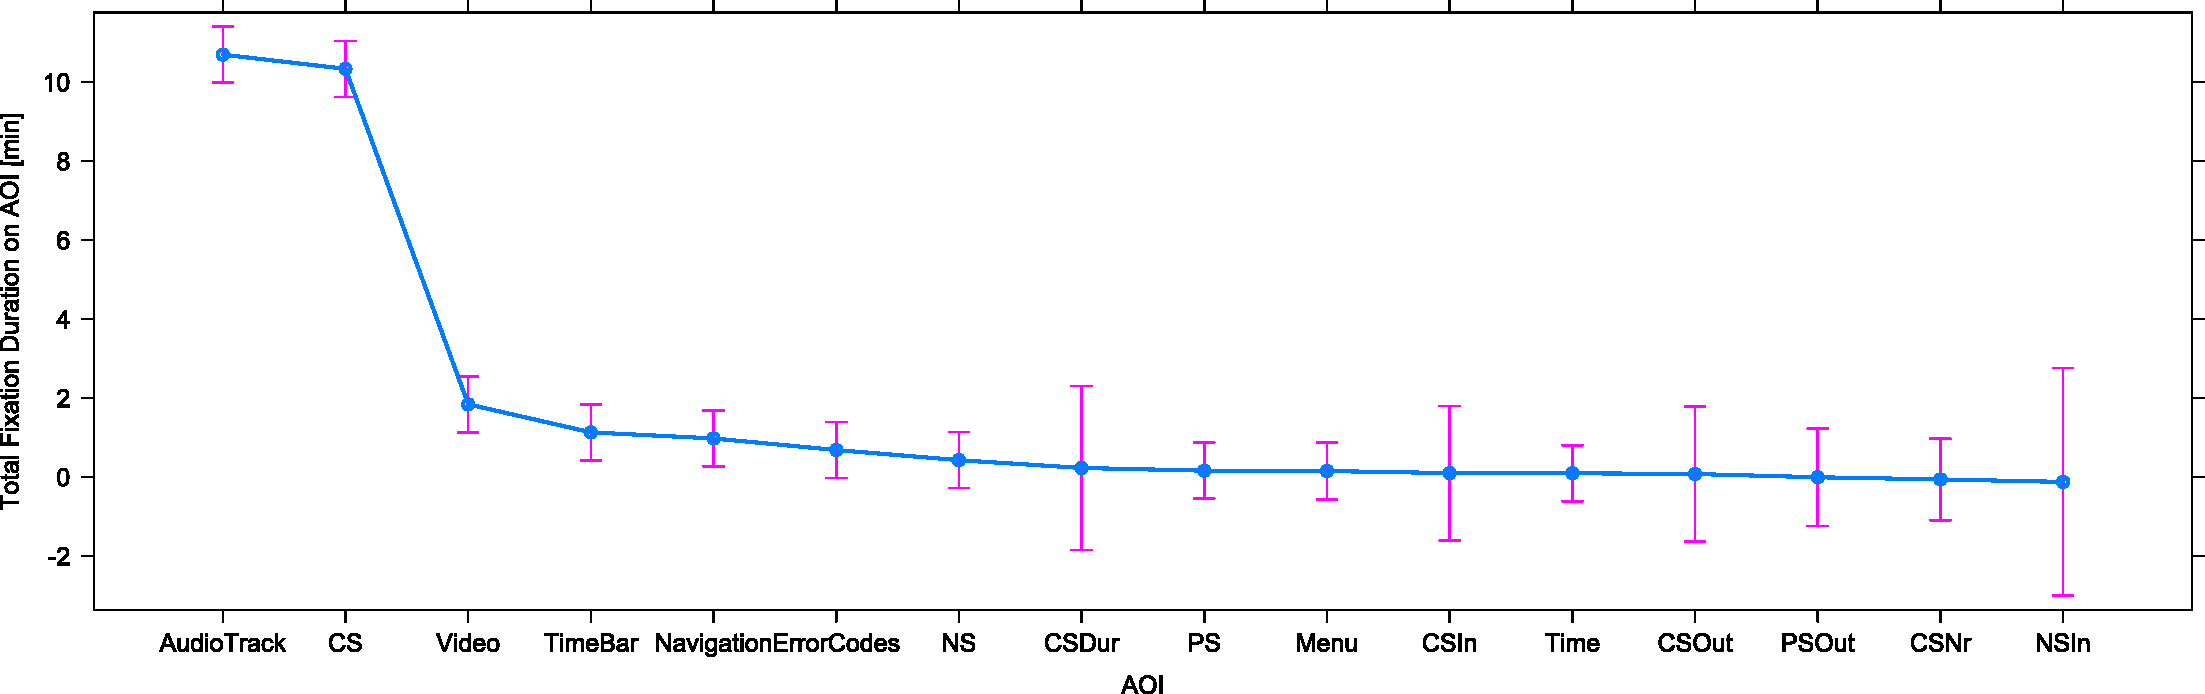
\includegraphics[width=1\textwidth]{figures/LME1_TotalFixDur_AOI.pdf}
%\includesvg[width=1\textwidth]{figures/LME1_TotalFixDur_AOI.pdf}
\caption{Effect of AOI on total fixation duration (in minutes)\label{fig:3_LME5}}
\end{figure}

Figure \ref{fig:3_LME5} visualises significant effects of the AOIs \textit{audio track} and \textit{current subtitle} (CS) on \textit{total fixation duration} in contrast to all other AOIs in FAB Subtitler.
With AOI \textit{video} as reference, the effects for \textit{audio track} ($\beta=8.9$, $\SE=0.4$, $\df=238$, $t=21.4$, $p<0.0001$) and \textit{CS} ($\beta=8.5$, $\SE=0.4$, $\df=238$, $t=20.5$, $p<0.0001$) were both highly significant and positive.

In a next step, we had a look at the average fixation duration on the different AOIs.
Both longer total reading time (TRT) and longer average fixation duration are indicative of increased cognitive effort while average fixation durations are in a certain sense an earlier measure than TRT.
Here, we found the highest average fixation duration for the AOI \textit{audio track}, the one AOI that did not have a significantly lower total fixation duration than AOI \textit{CS}, which is the subtitling area where the current subtitle is being typed and monitored.
Adjustments in the timing are done by listening to the \textit{audio track} and at the same time fixating the AOIs \textit{time bar} and \textit{error codes}.

An effects plot for the second LME is shown in Figure \ref{fig:4_LME4} with the AOIs ordered for their average fixation duration.
Here, we clearly see that \textit{CS} lies in the centre of the plot.
If we take AOI \textit{CS} as reference and look at the contrasts for \textit{average fixation duration} with the other AOIs, we find significant positive effects for \textit{audio track} ($\beta=382$, $\SE=40$, $\df=238$, $t=9.6$, $p<0.0001$) and \textit{error codes} ($\beta=196$, $\SE=40$, $\df=238$, $t=4.9$, $p<0.0002$) and the previous subtitle out time (\textit{PSOut}; $\beta=330$, $\SE=64$, $\df=241$, $t=5.2$, $p<0.0001$), i.e.
average fixation durations were significantly longer for these AOIs than on \textit{CS}.
Only marginally significantly shorter average fixation durations were found on the current subtitle ID (\textit{CSNr}; $\beta=-177$, $\SE=54$, $\df=239$, $t=-3.3$, $p<0.092$) and on the next subtitle (\textit{NS}; $\beta=-132$, $\SE=40$, $\df=238$, $t=-3.3$, $p<0.079$).
The AOI next subtitle only contains content when the subtitler has already created the proceeding subtitle and went back to check the preceding subtitle.
This indicates these areas might be processed faster than the current subtitle and seem to require less attention as also indicated by the first LME in Figure \ref{fig:3_LME5}.

\begin{figure}
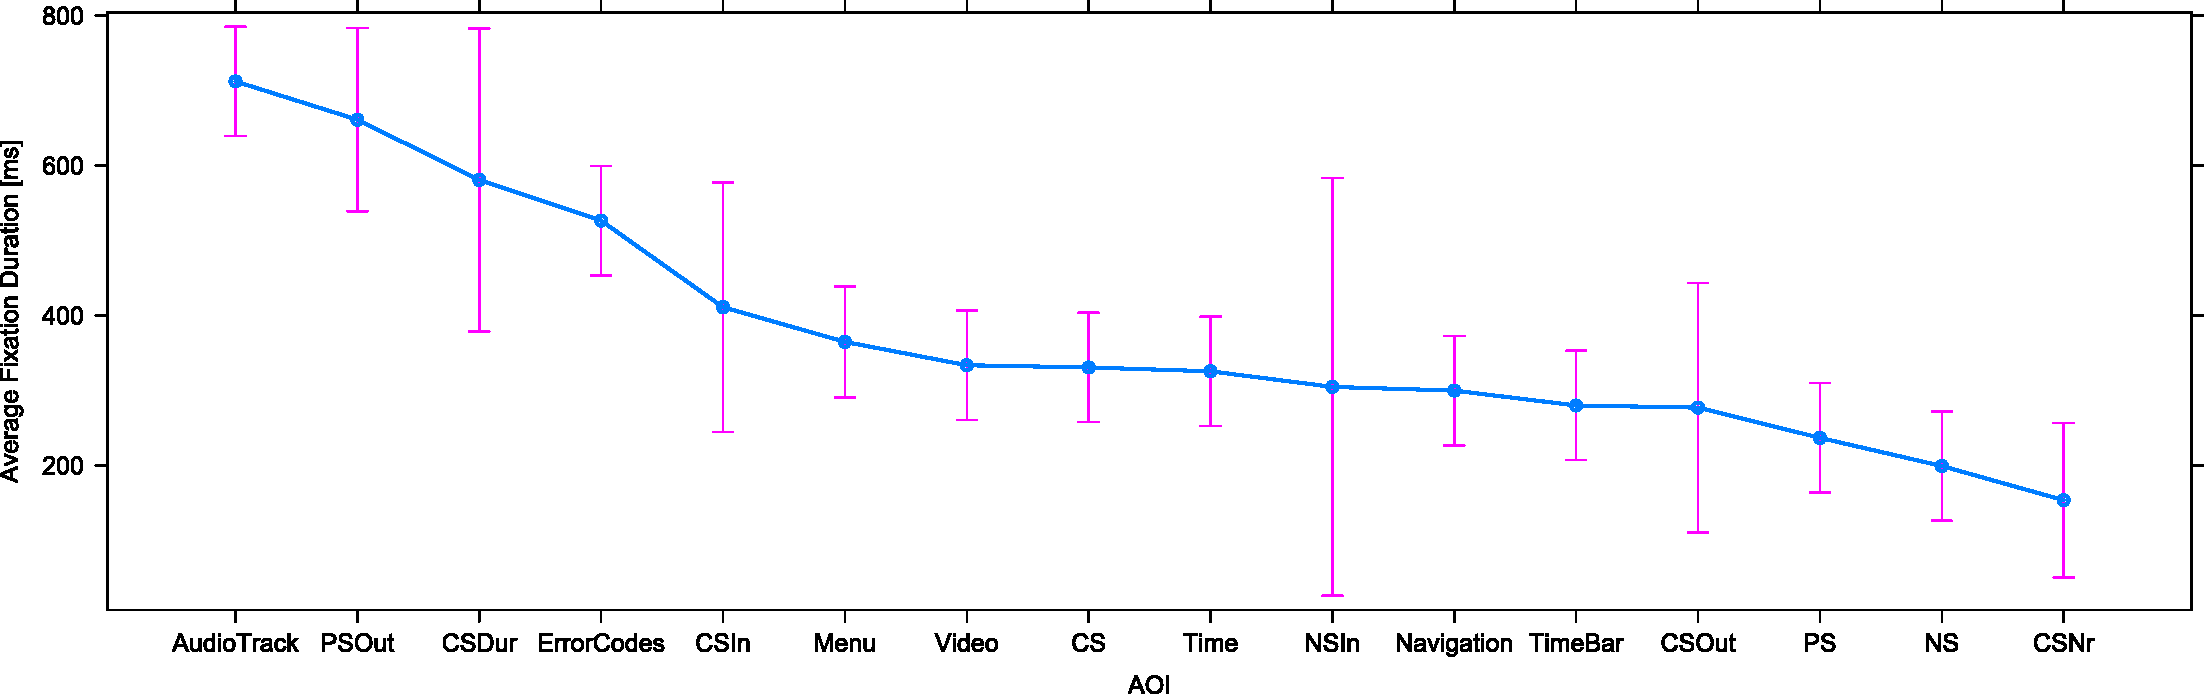
\includegraphics[width=1\textwidth]{figures/LME2_AvgFixDur_AOI.pdf}
%\includesvg[width=1\textwidth]{figures/LME2_AvgFixDur_AOI.svg}
\caption{Effect of AOI on average fixation duration (in milliseconds)\label{fig:4_LME4}}
\end{figure}
 
\subsection{Monitoring and cognitive load}
The second part of the analysis was concerned with the product of subtitling in relation to the process data.
Subtitles underwent post-experiment proofreading and were annotated if they contained some kind of error (Linguistic, Style or Timing).
In this first analysis, we did not differentiate between the nature of the error but simply whether a subtitle was correct or incorrect (\textit{Err}).

A plot for the first LME is shown in Figure \ref{fig:5_LME3}.
Here, we found a significant positive effect for the total reading time \textit{total fixation duration} for subtitles that still contained an error at the end of the session, i.e., subtitles that were edited during proofreading.
Subtitles which were corrected during proofreading (6 months after the experiment) were fixated longer during the subtitling session than subtitles which had not been corrected during proofreading ($\beta=0.9$, $\SE=0.28$, $\df=1680$, $t=3.3$, $p<0.001$), indicating that participants worked longer, or rather read these subtitles longer, yet failed to produce a correct subtitle.
This can be seen as an indicator that subtitles that resulted in an error required more attention than those subtitles that successfully followed the linguistic rules and the subtitle style guide.
\textit{Character count} was included in the model as a control variable and had a highly significant effect ($\beta=0.13$, $\SE=0.006$, $\df=1680$, $t=20.7$, $\smash{p<\num{2e-16}}$).

\begin{figure}
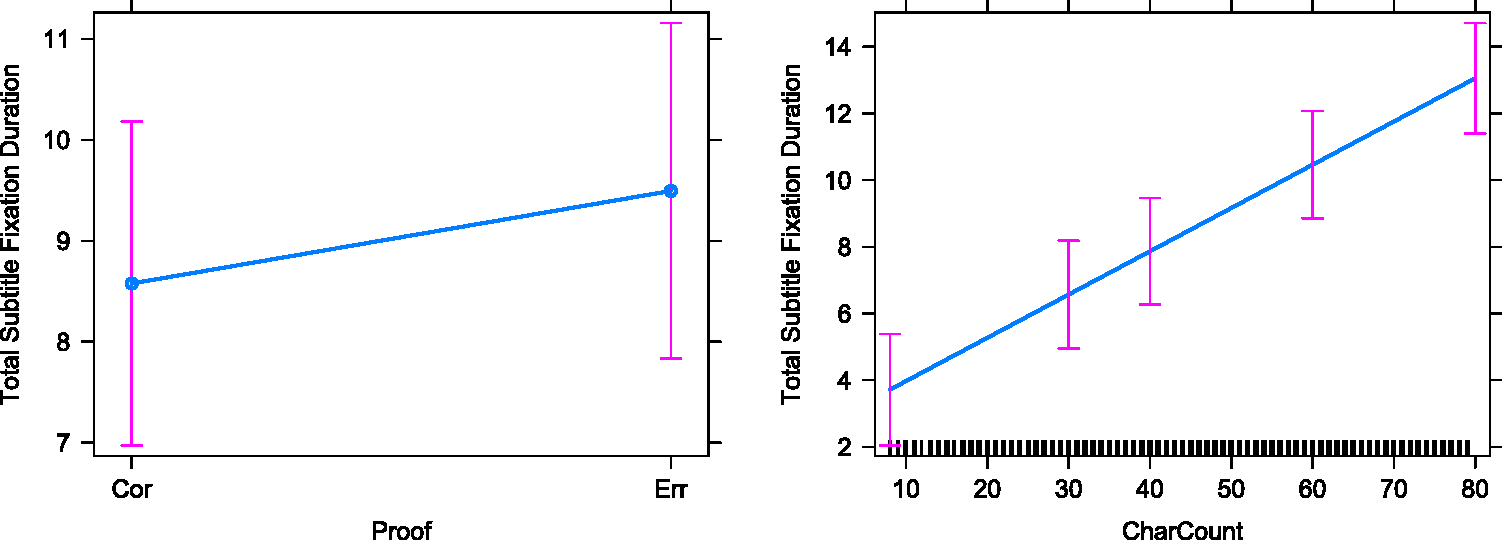
\includegraphics[width=1\textwidth]{figures/LME3_TotalFixDur_Proof.pdf}
%\includesvg[width=1\textwidth]{figures/LME3_TotalFixDur_Proof.svg}
\caption{Effect of proof and character count on the total subtitle fixation duration (in seconds)\label{fig:5_LME3}}
\end{figure}
 
We tested whether the sequential numbering of subtitles, which roughly corresponds to the time when the subtitle was produced (ID), would have an effect on the reading time.
The plot in Figure~\ref{fig:6_LME4} shows the positive effect of ID (numbered subtitles) on the reading time of the respective subtitle.
This means that during subtitling, participants spent significantly more time reading subtitles they created later in the session ($\beta=0.014$, $\SE=0.06$, $\df=1664$, $t=2.6$, $p<0.01$).
This also makes sense, as later in the session participants have concentrated and processed already quite a few subtitles and it can be assumed that cognitive load increases with time (if no break was taken).
 
\begin{figure}
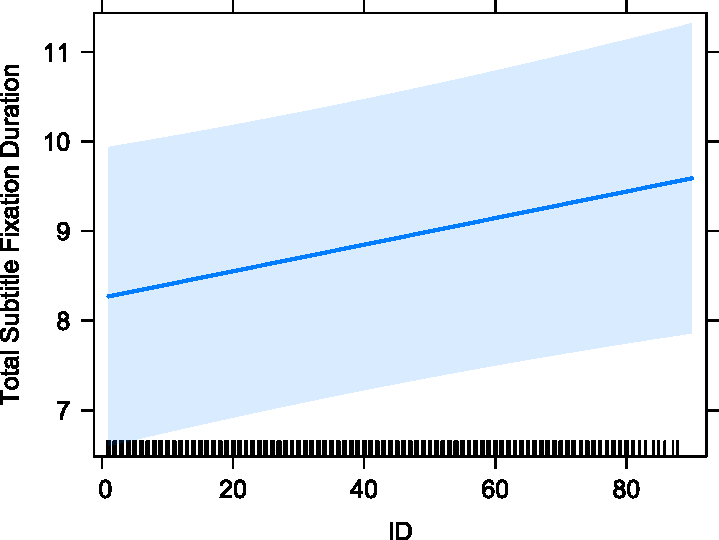
\includegraphics[width=0.5\textwidth]{figures/LME4_TotalFixDur_ID.pdf}
%\includesvg[width=0.5\textwidth]{figures/LME4_TotalFixDur_ID.svg}
\caption{Effect of ID, i.e.
whether a subtitle was created early in the session or later on Total Subtitle Fixation Duration (in seconds)\label{fig:6_LME4}}
\end{figure} 
 
After finding these two effects, we were curious whether the ID and the post-experiment annotation for the subtitles containing an error (timing, linguistic or style guide-related error) would interact.
Indeed, as can be observed in \figref{fig:7_LME5}, these two interact significantly ($\beta=-0.05$, $\SE=0.01$, $\df=1661$, $t=-4$, $p<0.001$) in that the reading times for subtitles later in the session did not differ significantly for correct and incorrect subtitles.
Additional analyses show that for subtitles annotated as correct, the effect of ID on the reading time was only marginally significant and positive ($\beta=0.03$, $\SE=0.01$, $\df=1662$, $t=4$, $p<0.001$).
For subtitles that contained some kind of error the effect of ID on reading time was significant and negative ($\beta=-0.03$, $\SE=0.01$, $\df=1661$, $t=-2$, $p<0.05$).
While we do find a significant difference in reading times for correct and incorrect subtitles early in the session, this difference disappears around two thirds into a session.

\begin{figure}
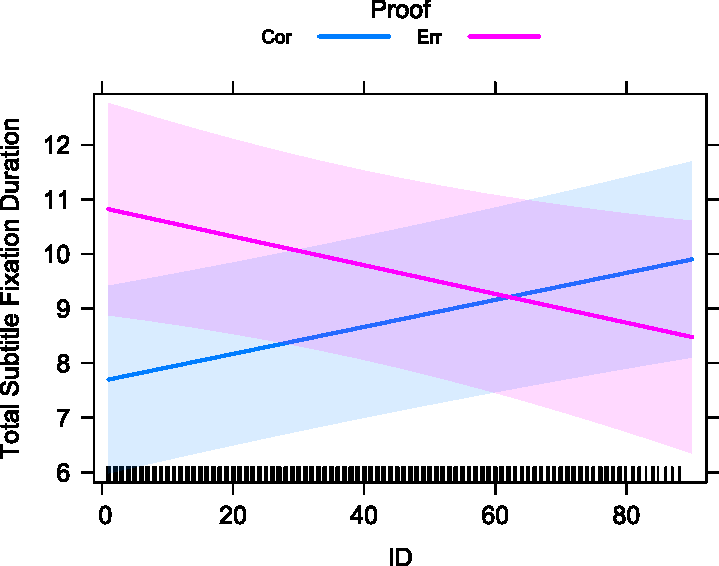
\includegraphics[width=0.5\textwidth]{figures/LME5_TotalFixDur_ID-Proof.pdf}
%\includesvg[width=0.5\textwidth]{figures/LME5_TotalFixDur_ID-Proof.svg}
\caption{Interaction effect of subtitle ID and post-experiment subtitle correction (proof) on total subtitle fixation duration (in seconds)\label{fig:7_LME5}}
\end{figure} 


In the next section, results will be interpreted and discussed regarding cognitive processing and monitoring during subtitling.

\section{Discussion} 
In cognitive load theory, gaze counts and gaze duration are regarded as established measures to quantify mental effort and cognitive load, which are, in turn, correlated with working memory capacities \citep{buettner2013}.
The methodological foundation for this measurement is corroborated by the eye-mind hypothesis, which assumes that information which is fixated with the eyes is immediately cognitively processed \citep{just1980theory}.
Based on this assumption, parameters like length, number or direction of the fixations, as well as reading time allow conclusions about cognitive load, on the one hand, but also on monitoring processes during translation, on the other \citep{carl-dragsted2012, schaeffer-etal2019}.
In the following, we will interpret our results against this background.

Figure \ref{fig:6_LME4} shows, for instance, that the total fixation duration increases the later a subtitle occurs in the whole subtitling session.
This can be interpreted as an indicator of increasing cognitive load, since the later subtitles require more visual attention to be processed compared to the early ones.
This result is not surprising since it may in turn be interpreted as increased cognitive load as a consequence of fatigue.

As mentioned above, for the purpose of this study, we adopted the concept of monitoring by \citet{kitchener1983cognition} and defined subtitles with errors as ill-structured problems that trigger monitoring processes while reading them.
Keeping this definition in mind, Figure \ref{fig:6_LME4} can be interpreted as an indicator for ongoing monitoring processes that add up during the session.
In this special case, the subtitlers' total fixation duration is positively affected by the ID, i.e. later in the session the total fixation durations were longer, when the subtitle they produced still contained an error (see Figure \ref{fig:5_LME3}).
However, this effect is not triggered by correction processes as the respective subtitles have not been self-corrected by the subtitlers or, if they have, still resulted in an error.
More interestingly, the effect seems to be triggered while creating the particular subtitle.
Therefore, we interpret this effect as increased cognitive load due to monitoring.

Figure \ref{fig:7_LME5} shows another interesting phenomenon: the monitoring effect just described seems to be weakened throughout the reading during subtitling.
As soon as about two thirds of the subtitles are processed, the total fixation duration for correct subtitles is even longer.
We interpret this result as follows: monitoring of subtitles that did not follow the style guide, hence contained some kind of error, can only take place in the first half of the subtitling session when necessary cognitive resources are still available.
If these resources suffer from fatigue, the monitoring processes for incorrect subtitles do not differ from those of correct ones, which are in general characterised by shorter total fixation duration.
This could indicate cognitive overload since incorrect subtitles do not attract as much visual attention anymore.

To sum up, the effects discussed here make monitoring visible although no successful revision processes have taken place.
This enables us not only to visualise but also to quantify possibly unconscious monitoring processes as well as the break-even point for cognitive overload.

\section{Conclusion and limitations}
As discussed in the section above, with this small-scale pilot study we were able to obtain a first idea of when and where monitoring processes in intralingual subtitling might take place and we presented a methodology of how these processes can be studied when linked to final target text quality.
In this analysis, we looked at two measures: total and average fixation duration per subtitle or AOI.
We find that further into the session , monitoring becomes less efficient and participants generally read subtitles longer irrespective of the number of characters they contain.
While earlier in the session subtitlers take longer for subtitles that result in an error, this difference is no longer significant towards the end of the session.
This suggests that, due to increased cognitive load, subtitlers' monitoring processes become less or not successful at all.

Still, this study was able to shed light on monitoring processes during subtitling.
\citet{ipsen-dam2016} also report on errors detected but not corrected.
They, in contrast, rely on video recordings and interviews, which reveal conscious and explicitly visible processes.
In our study, unconscious language control mechanisms become for the first time visible and measurable.
By combining eye tracking with further data from keylogging and retrospective interviews with replay we might be able to cover both conscious as well as unconscious processes and deliver explanations for unsuccessful revision processes in future studies.

Based on these findings, the aim of a subtitling tool should be to improve monitoring for subtitlers or make these language control mechanisms more efficient.
In this respect, the usability of the tool has a direct impact on the cognitive ergonomic conditions during professional translation \citep{ehrensberger2014cognitive}.
Subtitling software, just like computer-aided tools for professional translation, are developed to assist the tasks in terms of an ergonomic workflow.
However, the usability of these tools has so far not been empirically tested.
The  features included in the tools seem necessary and helpful but right now our results suggest that this assisting technology has room for improvement, e.g.
error messages regarding incorrect timing are not easily detected -- especially later in the process -- and errors regarding segmentation or linguistic problems are overlooked.
The methodology and study design presented in this paper could be useful in comparing subtitling software that claims to be more ergonomic (e.g. the Compass tool, \citealt{hansen-schirra-etal2019}).

The results presented here are somewhat limited due to the small sample size as well as the nature of the experiment as participants subtitled only short excerpts from the documentaries.
Subtitling sessions usually take longer than an hour, but already finding significant results in these shorter sessions suggests that these effects might hold true also for longer sessions.
If we consider subtitlers' authentic work spaces and the complex workflows of replaying and stopping the videos to type and spot the subtitles according to the complex style guides, it makes sense to further investigate these processes.
The methodology applied in the experiment was conducted with rather high ecological validity such that the results hold true beyond the lab environment.
We hope the successful application of this methodology and the resulting insights encourage further research in this direction with other subtitling tools, languages, style guides or practices.

\section*{Acknowledgements}
The Compass project received funding from the European Union within the call \textit{Crowdsourcing subtitling to increase the circulation of European works} (CNECT 2017/3135124) from 2018--2019.

{\sloppy\printbibliography[heading=subbibliography,notkeyword=this]}
\end{document}
